%  Copyright (C) 2002 Regents of the University of Michigan, portions used with permission 
%  For more information, see http://csem.engin.umich.edu/tools/swmf
%\documentclass[12pt]{revtex4}
%\usepackage{graphicx}
%\begin{document}
%\title{ N-temperature model}
%\begin{abstract}
\section{Appendix D: How to solve coupled system of N temperature equations.} 
The numerical solution of the non-linear heat conduction problem in the
coupled system of the energy equations (say, for internal energy of radiation, 
electrons and/or ions) is reduced to a numerical solution of the system of linear 
equations with a sparse matrix, which is symmetric, definite positive and 
diagonal-dominant.
%\end{abstract}
%\maketitle 
\subsection{Governing equations and their symmetry}
Consider the coupled system of the energy equations as follows:
\begin{equation}\label{gov}
\frac{\partial {\cal E}_\alpha}{\partial t}=
\nabla\cdot\left(\kappa_\alpha\nabla T_\alpha\right)+
\sum_{\beta\ne\alpha}
{R_{\alpha\beta}(T_\beta-T_\alpha)},
\end{equation}
where $\cal E$ is the internal energy density, index $\alpha=1,...,N$ enumerates $N$ 
different components involved into a consideration, such as plasma as a 
single component or electrons and ions as two separate components and/or radiation; 
$T_\alpha$ being the temperature of the component (for radiation 
$aT^4_r={\cal E}_r$, hence, $T_r= ({\cal E}_r/a)^{1/4}$); the heat fluxes 
are assumed to have a form of
$-\kappa_\alpha\nabla T_\alpha$; and $R_{\alpha\beta}$ 
characterizes the rate of energy exchange between different components. For 
gray radiation absorbtion the latter coefficient is:
\begin{equation}
R_{re}=\frac{c k_p(aT_e^4-E_r)}{T_e-T_r}=c k_p a(T_e+T_r)(T_e^2+T_r^2),
\end{equation}  
where $k_p$ is the Planck opacity. Note also that in analogous manner the diffusive
flux of the gray radiation energy, which is usually expressed in terms of the radiation
energy density gradient, $\nabla{\cal E}_r$, may be reduced to the form as in 
Eq.(\ref{gov}), because $\nabla{\cal E}_r=4aT^3_r\nabla T_r$. All the variables and 
parameters
may be dependent on temperatures as well as on the other plasma parameters (density, ionization degree etc)
\subsection{Symmetry and positivity}
In accordance with the second law of thermodynamics, the heat always transferred from 
the body with higher temperature to that with lower one, so that:
\begin{equation}\label{pos}
\kappa_\alpha\ge0,\,\,\,R_{\alpha\beta}\ge0.
\end{equation}
Another property of the governing equations comes from the detailed equilibrium 
principle which relates the energetic rates for direct and reverse processes
and requires, that:
\begin{equation}\label{sym}
R_{\alpha\beta}=R_{\beta\alpha}.
\end{equation}
In particular, Eq.(\ref{sym}) ensures the total energy conservation:
$\frac{d}{dt}\sum_\alpha{\int{{\cal E}dV}}=0$, 
because on the right hand side of Eq.(\ref{gov}) the divergence of the heat flux vanishes in integrating
over a volume, while the energy exchange rates cancel each other locally on suming by $\alpha$.
\subsection{Discretization}
%Leaving for the further discussion the issue of dscretizating the time derivatives in 
%Eq.(\ref{gov}), 
Consider the semi-discrete set of equations, obtained by 
applying the finite volume formulation to Eq.(\ref{gov} ) and employing the set of 
control volumes, $V_i$, enumerated by a single index, $i=1,...,I$:  
\begin{equation}\label{sem}
V_i\frac{d {\bf E}_i}{d t} + \sum{{\bf F}_{ij}}+V_i{\bf R}_i\cdot {\bf T}_i=0,
\end{equation}
Here the elements $E_{\alpha i}$ of the state vector in the $i$th volume are the 
averaged value of the energy density, ${\cal E}_\alpha$. The %elements of the 
fluxes, 
%vector, 
$F_{\alpha ij}$ may be obtained by approximating the temperature gradient: 
$F_{\alpha ij}= \kappa_{\alpha ij}S_{ij}(T_{\alpha i}- T_{\alpha j})/\|x_i-x_j\|$. The 
index $j$ enumerates the control volumes which have the common face with the $i$th 
control volume, the face area being $S_{ik}$ and the distance 
between the cell centers being $\|x_i-x_j\|$.
%
%Now discuss the relaxation matrix, ${\bf C}_i$. Unlike the other bold-font variables
%which all are $N$-vectors, for a given volume or a given face, the relaxation matrix is
%$N*N$ matrix, which for a given control volume describes the local rates of the 
%energy exchange between the components. 
The elementss of $N*N$ matrix, ${\bf R}_i$, are: 
$-R_{\alpha\beta i}$, for off-diagonal elements ($\alpha\ne\beta$), and 
$\sum_{\beta\ne\alpha}R_{\alpha\beta i}$,
for the $\alpha$th diagonal element.

All the coefficients and variables in Eq.(\ref{sem}), again, may be highly non-linear 
functions of 
temperature. However, now we employ the {\it principle 
of frozen coefficients}. Specifically, in advancing the solution 
through a time %interval 
%$(t^n,t^{n+1})$, which is the time 
step, 
$\Delta t=t^{n+1}-t^n$, we assume all the coefficients, 
$\kappa_{\alpha ij}$ and ${\bf R}_i$ to be constant in time and keep their values as 
in the time instant, $t^n$. Moreover, we
also approximate the time derivative of ${\cal E}_\alpha$ in terms of that of 
temperature, 
$\partial{\cal E}_\alpha/\partial t = C_\alpha \partial T_\alpha/\partial t$, where 
$C_\alpha=\partial {\cal E}_\alpha/\partial T_\alpha$ is the specific heat. Thus, 
Eq.(\ref{sem}) becomes:
\begin{equation}\label{lin}
V_i{\bf diag}\{C_\alpha\}_i\cdot\frac{d{\bf T}_i}{d t} +\sum_j{\frac{S_{ij}
{\bf diag}\{\kappa_{\alpha ij}\}\cdot
\left({\bf T}_i-{\bf T}_j\right)}{\|x_i-x_j\|}}+V_i{\bf R}_i\cdot {\bf T}_i=0,
\end{equation}
where ${\bf diag}\{C_\alpha\}$ denotes $N*N$ matrix with the diagonal 
$\alpha\alpha$ element being  $C_\alpha$. % and all off-diagonal elements being equal to 
%zero.  %is a system of linear differential equations with respect to 
%temperatures. 
Now we advance the solution of Eq.(\ref{lin}) through the time step using fully 
implicit scheme. To achieve this, one needs to solve a linear system as follows:
\begin{eqnarray}
\frac{V_i{\bf diag}\{C_\alpha\}_i
\cdot{\bf T}^{n+1}_i}{\Delta t}+\sum_j{\frac{S_{ij}
{\bf diag}\{\kappa_{\alpha ij}\}\cdot
\left({\bf T}^{n+1}_i-{\bf T}^{n+1}_j\right)}{\|x_i-x_j\|}}+\nonumber\\
+V_i{\bf R}_i\cdot {\bf T}^{n+1}_i
=\frac{V_i{\bf diag}\{C_\alpha\}_i\cdot{\bf T}^{n}_i}{\Delta t}.\label{alg}
\end{eqnarray}
The left hand side of this equation is the product, ${\bf A}\cdot{\bf T}^{n+1}$, of the $I*I$ block matrix, 
${\bf A}_{ij}$, the elements of the block matrix being $N*N$ matrices, with the block $I$-vector, 
${\bf T}^{n+1}_i$, the elements of the block vector being $N$-vectors. In the matrix ${\bf A}$ all 
off-diagonal blocks are diagonal $N*N$ matrices: 
\begin{equation}
{\bf A}_{ij}={\bf A}_{ji}=-\frac{S_{ij}
{\bf diag}\{\kappa_{\alpha ij}\}}{\|x_i-x_j\|},\,\,i\ne j.
\end{equation}
We see that the off-diagonal block part of the matrix ${\bf A}$ is symmetric and all numbers in 
this part are non-positive, according to Eq.(\ref{pos}). The diagonal blocks are:
\begin{equation}
{\bf A}_{ii} = \frac{V_i{\bf diag}\{C_\alpha\}_i}{\Delta t} -\sum_{j\ne i}{{\bf A}_{ij}} +V_i {\bf R}_i.
\end{equation}
The off-diagonal elements in the matrix ${\bf R}_i$ are again symmetric and non-positive, due to
Eqs.(\ref{pos},\ref{sym}). Hence, the matrix ${\bf A}$ is symmetric. It is also diagonal-dominant: 
taking the difference %, $A_{\alpha\alpha ii}-\sum_{\beta\ne\alpha}{|A_{\alpha\beta ii}|}-\sum_{i\ne j}{|A_{\alpha\alpha ij}|}$, 
between the diagonal element and the sum of absolute values of all off-diagonal 
elements in the same line, one can see, that:
\begin{equation}
A_{\alpha\alpha ii}-\sum_{\beta\ne\alpha}{|A_{\alpha\beta ii}|}-\sum_{i\ne j}{|A_{\alpha\alpha ij}|}=\frac{V_iC_{\alpha i}}{\Delta t} >0.
\end{equation}
Thus, we proved that the matrix ${\bf A}$ is symmetric and diagonal-dominant. As a consequence,  it is positive definite, but the diaginal 
domination is more strong and usefull property. There is a variety of tools
allowing to solve efficiently the system of equations with such kind of matrices, for example, preconditioned conjugated gradients.

Finally, we show how to employ ${\bf T}^{n+1}$ found from non-conservative Eq.(\ref{lin}) to advance the solution of original 
Eq.(\ref{sem}), which conserves the energy. To do this, one needs to express the fluxes and energy in Eq.(\ref{sem}) in terms of
${\bf T}^{n+1}$, still keeping the coefficients frozen. After a simple algebra we obtain:
\begin{equation}\label{con}
{\cal E}_{\alpha i}^{n+1} = {\cal E}_{\alpha i}^{n}+C_{\alpha i}(T^{n+1}_{\alpha i}-T^n_{\alpha i}).
\end{equation} 
The corrected temperature at the time instant $t^{n+1}$ then should be recovered from ${\cal E}$ using the equation of state, and,
for plasma with the temperature-dependent specific heat. it may differ from $T^{n+1}$.  
Note also that at this final stage, theoretically, the choice of too large time step may result in negative temperature. Indeed, although ${\bf T}^{n+1}$ 
are all positive, it is not guaranteed that at $T^{n+1}\ll T^{n}$ the energy ${\cal E}^{n+1}$ found from Eq.(\ref{con}) exceeds the value corresponding to
zero temperature. The advance through the timestep in this case may be done in two stages, getting the temperature drop limited.
\begin{figure}
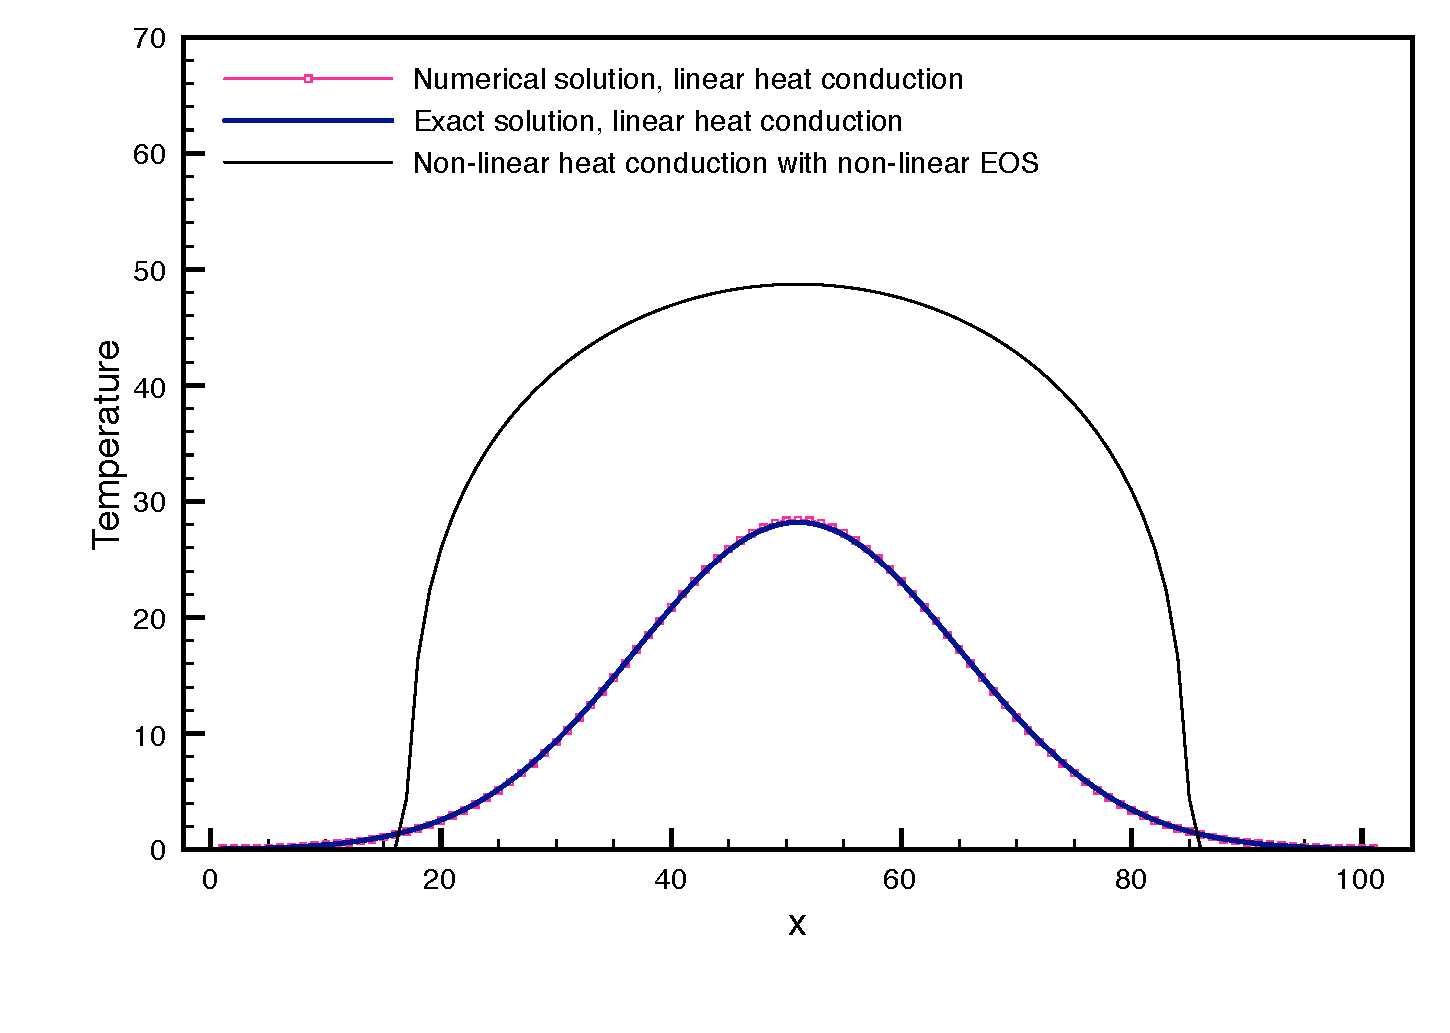
\includegraphics[scale=0.50]{Fig1.eps}
\caption{The test result for N-temperature model using conjugeted gradients method with Jacobi block preconditioner (${\bf A}_{ii}$ matrix is 
exactly inverted): (1) linear heat conduction equation compared with the anylitical solution  (to test the CG routine) and the numerical solution 
of the non-linear heat conduction equation is compared to that of the coupled system of heat conduction with very high energy exchange rate 
(1000 per time step) and the same total conduction and heat capacity as for a single equation. Not surprisingly, the solution of the strongly coupled 
system is not different from that for a single equation, but remarkable is the fact that such the high energy exchange rate does not affect
the iteration convergence rate.
}
\label{fig_1}
\end{figure}  
\subsection{Generalizations: $N+M$ temperatures, and temperature powered $n$.}
Note some more or less trivial generalizations of the developed approach. 

{\bf Non-linear temperature.} So far we considered only the temperaature values for different components of the physical system, as the unknowns to be solved 
numerically. However, in many problems of the thermodynamics the term ``temperature'' implies ``...or any monotonous function on it''. Particularly any 
monotonous function of temperature, $T_{\rm new}(T)$ can be introduced instead of the the temperature, into the governing equations or into the finite volume 
formulation. In the latter 
case while setting the frozen coefficients the {\it Lipshitz derivative} should be used, which is the symmetric positive function, $T_{\rm new}^\prime(T_1,T_2)$, of two 
input parameters, $T_1$ and $T_2$, such that for any $T_1$ and $T_2$, by definition,
\begin{equation}
T^\prime_{\rm new}(T_1,T_2)=\frac{T_{\rm new}(T_1)-T_{\rm new}(T_2)}{T_1-T_2}.
\end{equation}   
Particularly, for the power law $T_{\rm new}(T)=aT^L$ with the integer index, $L$, the Lipshitz derivative is 
$T_{\rm new}^\prime(T_1,T_2)=a\sum_{l=0}^{L-1}{T^{L-1-l}_1T_2^l}$. The system of linear equations, (\ref{alg}), as formulated in terms of $T^{n+1}_{\alpha i}$, has the 
same form as before, bur the frozen coefficients in it are frozen in a different way:
\begin{equation}
C_{\alpha i}\rightarrow \frac{C_{\alpha i}}
{T^\prime_{\rm new}(T^n_{\alpha i},T^n_{\alpha i})},\qquad
R_{\alpha\beta i}\rightarrow \frac{R_{\alpha\beta i}}
{T^\prime_{\rm new}(T^n_{\alpha i},T^n_{\beta i})},
\end{equation} 
\begin{equation}
\kappa_{\alpha ij}\rightarrow \frac{\kappa_{\alpha ij}}
{T^\prime_{\rm new}(T^n_{\alpha i},T^n_{\alpha j)}},
\end{equation}
Positivity, symmetry and the diagonal domination are proved in the same way as above, using the positivity ond symmetry of the Lipshitz derivative. Since the
Lipshitz derivatives are taken as the frozen coefficients, the non-linear temperature approach implies another choice of the linerization procedure in the 
governing equations. 

{\bf Partial inversion of the advancing operator} may or may not make sense, if the heat transfer for one or some of the physical components is negligible (for, example 
the ion heat conduction usually, but not always, is small as compared with the electron one).  In this case one can re-write Eq.(\ref{alg}) in the following manner, which
lists only $N$ equations including heat conduction, with extra term describing the energy exchange with $M$ non-heat-conducting components, for which the
temperature is denoted as $\Theta_{Mi}$ and the enumerating index for these components is denoted with upper case $M$ :
\begin{eqnarray}
\frac{V_i{\bf diag}\{C_\alpha\}_i
\cdot{\bf T}^{n+1}_i}{\Delta t}+\sum_j{\frac{S_{ij}
{\bf diag}\{\kappa_{\alpha ij}\}\cdot
\left({\bf T}^{n+1}_i-{\bf T}^{n+1}_j\right)}{\|x_i-x_j\|}}+\nonumber\\
+V_i{\bf R}_i\cdot {\bf T}^{n+1}_i %+ V_i{\bf diag}\{\sum_M{R_{\alpha Mi}} \}\cdot 
%{\bf T}^{n+1}_i 
-  V_i\|R_{\alpha M}\|_i\cdot{\bf \Theta}_i^{n+1}
=\frac{V_i{\bf diag}\{C_\alpha\}_i\cdot{\bf T}^{n}_i}{\Delta t}.\label{NM}
\end{eqnarray}
Note that the diagonal elements of the ${\bf R}$ matrix includes a 
contribution from the energy exchange between heat-conducting and non-heat-conducting components. Analogously, 
$M*M$ ${\bf r}_i$ matrix for the
energy exchange between non-heat-conducting components also includes the diagonal elements accounting for the contributions from heat-conducting components. 
The equation  for non-heat-conducting components reads:
\begin{equation}
\frac{{\bf diag}\{C_M\}_i
\cdot{\bf \Theta}^{n+1}_i}{\Delta t}+
{\bf r}_i\cdot {\bf \Theta}^{n+1}_i %+ {\bf diag}\{\sum_\alpha{R_{M\alpha i}} \}\cdot 
%{\bf \Theta}^{n+1}_i 
-  \|R_{ M \alpha}\|_i\cdot{\bf T}_i^{n+1}
=\frac{{\bf diag}\{C_M\}_i\cdot{\bf \Theta}^{n}_i}{\Delta t}.\label{MN}
\end{equation}

All this derivations make sense as long as the matrix of the advancing operator in Eq.(\ref{MN}) may be inverted, to find:
\begin{equation}
{\bf B}_i^{-1}=\left(\frac{{\bf diag}\{C_M\}_i}{\Delta t}+{\bf r}_i\right)^{-1}.
\end{equation}
Using the inverted matrix, one can exclude ${\bf \Theta}^{n+1}_i$ from (\ref{NM}) using the following equation:
\begin{equation}
{\bf \Theta}^{n+1}_i={\bf B}_i^{-1}\cdot\left(\frac{{\bf diag}\{C_M\}_i\cdot{\bf \Theta}^{n}_i}{\Delta t}+ \|R_{ M \alpha}\|_i\cdot{\bf T}_i^{n+1}\right).\label{solveM}
\end{equation}
On excluding ${\bf \Theta}^{n+1}_i$ Eq.(\ref{NM}) again takes the form of Eq.(\ref{alg}) with the following modifications:
\begin{eqnarray}
{\bf R}_i\rightarrow {\bf R}_i-\|R_{\alpha M}\|_i\cdot{\bf B}_i^{-1}\cdot\|R_{\alpha M}\|_i,\nonumber\\%qquad, 
{\bf diag}\{C_\alpha\}_i\cdot{\bf T}^{n}_i\rightarrow 
{\bf diag}\{C_\alpha\}_i\cdot{\bf T}^{n}_i+\|R_{\alpha M}\|_i\cdot{\bf B}_i^{-1}\cdot {\bf diag}\{C_M\}_i\cdot{\bf \Theta}^{n}_i.\label{solveN}
\end{eqnarray}
So, the detailed algorithm in this case may be as follows: (1) in each point, $i$, find the inverted matrix ${\bf B}_i^{-1}$; (2) modify the matrix of the equation
for heat-condicting components using (166); (3) solve Eq.(\ref{alg}), with the modified relaxation matrices and changed right hand side, througout the
whole computational domain; (4) at each point solve temperatures for non-heat-condicting components, using (165). The symmetry of the modified matrix ${\bf R}$ is
evident, less evident is its diagonal domination. The latter is a consequence of the above mentioned contributions from the cross interactions, into the diagonal elements of 
${\bf R}$ and ${\bf r}$ matrices.


\subsection{Summary}
Thus, to update the conservative system of non-linear heat conduction equations one needs: (1) to calculate coeffecients in the matrix ${\bf A}$, 
(2) solve the predicted values of temperature from the system of linear equations with symmetric, positive definite and diagonal-dominant matrix, 
(3) update the energy using Eq.(\ref{con})

%\end{document}

